\documentclass[landscape]{a0poster} 

% encoding and font
\usepackage[utf8]{inputenc}
\usepackage[T1]{fontenc}
\usepackage{lmodern}
\usepackage[english]{babel}

% Geometry
\usepackage{geometry}
\geometry{top=2cm, bottom=2cm, left=2cm, right=2cm}

% Fonts and visuals
\usepackage{graphicx, color, xcolor}
\usepackage{multicol}
\usepackage{amsmath, amssymb}
\usepackage{booktabs}
\usepackage{enumitem}
\usepackage{titlesec}
\usepackage{caption}
\usepackage{pgfplots}
\pgfplotsset{compat=1.18}

% Charts and diagrams
\usepackage{tikz}
\usepackage{pgf-pie}

% Fonts
\usepackage{sourcecodepro}
\renewcommand{\familydefault}{\sfdefault}

% Header
\usepackage{fancyhdr}
\pagestyle{fancy}
\fancyhf{}
\lhead{BitTorrent Distributed Systems}
\rhead{Leon Example}
\renewcommand{\headrulewidth}{1pt}

% Section formatting
\titleformat{\section}{\Large\bfseries\color{blue}}{}{0em}{}
\titleformat{\subsection}{\large\bfseries\color{black}}{}{0em}{}

% URL support
\usepackage{hyperref}

% Load custom layout helpers
\usepackage{PosterTemplates}

\begin{document}

% Title Banner
\maketitlebar{How BitTorrent Optimises Distributed Systems for Peer-to-Peer File Transfers}

\begin{multicols*}{3}

  \addsection{What is BitTorrent?}
BitTorrent is a peer-to-peer protocol and software for sending files over the internet, which allows users to send large files over the internet by connecting multiple sources at the same time, rather than relying on a single server to do it instead [1].

\addsection{Why do we need it? Limitations of traditional file transfer}
Traditional methods like email or FTP lack any security and have limited data sharing. This can lead to data inconsistency and redundancy. These methods also struggle with larger file sizes and complex data sharing. Other methods like using centralised servers, also introduce problems like single points of failure, potential data loss or corruption and many more [2].

\addsection{Importance of distributed systems and P2P architecture}
Distributed systems are an essential part for today’s modern computing needs, with their abilities such as enhanced scalability, fault tolerance and other factors that make them great for handling large-scale data transfer and processing. The P2P architecture allows our distributed systems to eliminate central authority by allowing nodes to function both as clients and servers, which then improves the systems resilience to faults as there no longer is a single point of failure. It also further improves scalability as new nodes are able to seamlessly be joined into the network [3].

\addfigure{img/p2p.png}{Diagram of P2P systems [4].}

\addsection{How BitTorrent Works}
Bittorrent works by locating other computers using the same software that have the file you wish to download. These other computers are ordinary computers like your own that are known as peers.
The process starts by finding a link for the file you want. Your bittorrent client software will then communicate with a tracker to find other computers running BitTorrent that have the complete file (known as seed computers) and those with portions of the file, these are typically peers in the process of downloading said file. The tracker identifies the swarm, which is a group of connected computers that have all or a portion of the file and are also in the process of sending or receiving it. The tracker then helps trade pieces of the file you want with others in the swarm, you can also receive multiple pieces of the files at once [5].

\addfigure{img/torrentdiagram.png}{Diagram of how torrents work [5].}

\addsection{Performance Comparison}
BitTorrent scales better than traditional  client-server systems because each peer contributes bandwidth. Performance improves as the swarm grows, making it ideal for large-scale distribution. It also offers resilience — if one peer fails , others still maintain availability. In contrast, centralized servers  present single points of failure and bottlenecks under load [6].

\begin{center}
  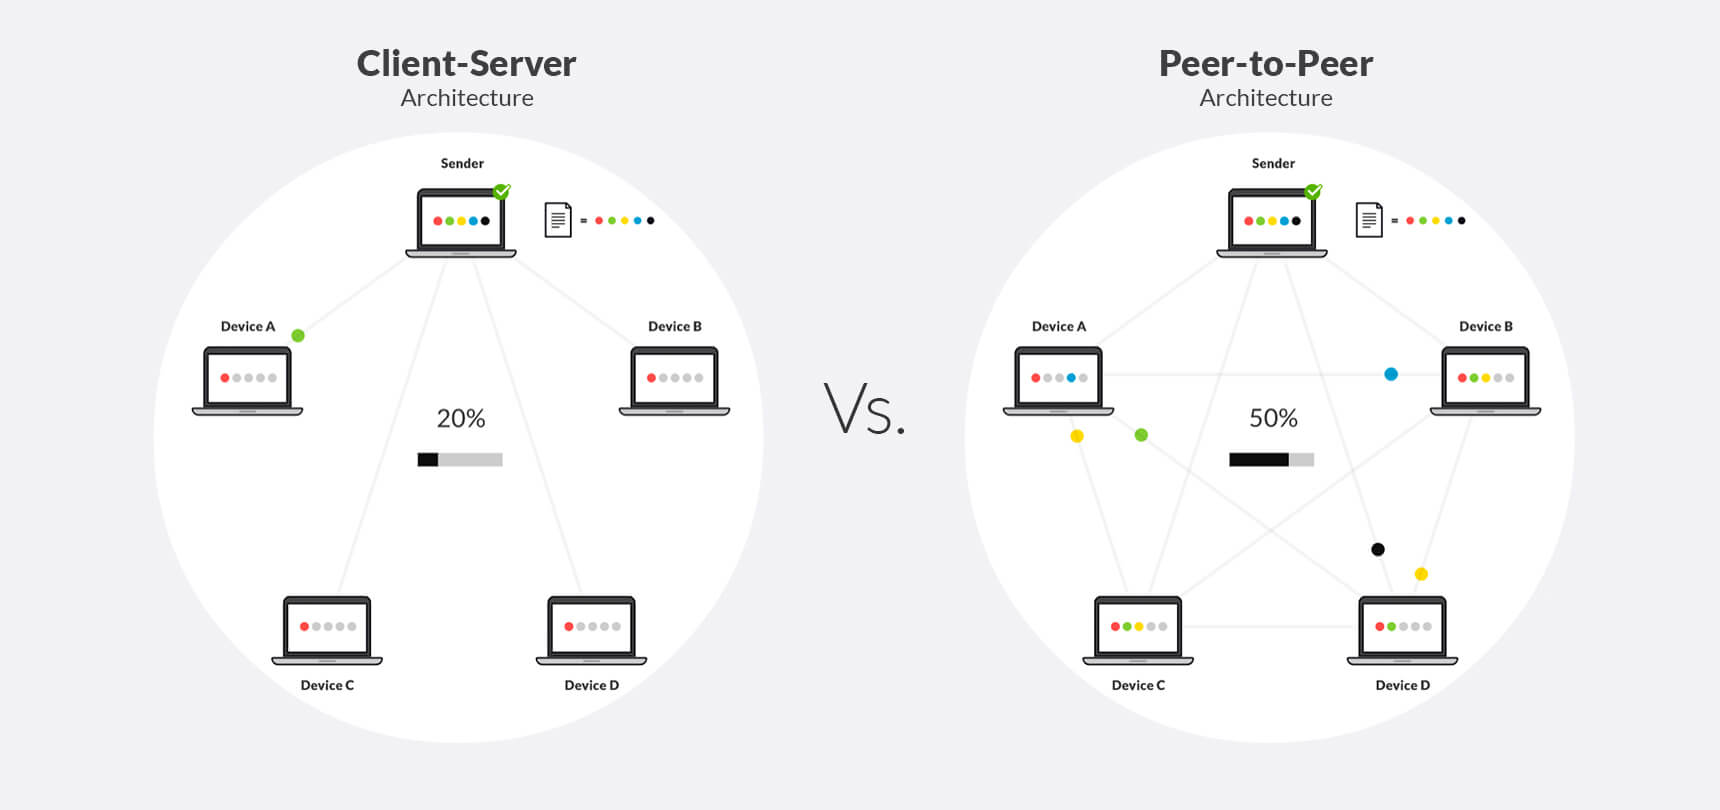
\includegraphics[width=1\linewidth]{img/comparison.jpg} \\
  {\footnotesize Comparison of the client-server system vs peer-to-peer system [6].}
\end{center}

\addsection{Real-World Applications}

\textbf{  Open-Source Distribution} \\
BitTorrent is widely used by open-source communities to distribute  large files. Linux distributions such as Ubuntu and Fedora rely on the protocol to share installation ISOs efficiently, minimizing server bandwidth and encouraging  community participation through seeding [7].

\vspace{1em}

\textbf{Gaming and Software Delivery} \\
Companies like Blizzard Entertainment have leveraged  BitTorrent to deliver large-scale game updates and patches to millions of users. The protocol helps manage high demand while maintaining  fast and reliable distribution [7].

\vspace{1em}

\textbf{Enterprise Use} \\
Facebook previously employed a customized BitTorrent  client to deploy code across its global data centers. This decentralized approach allowed faster  and more resilient internal software rollouts [7].

\vspace{1em}

\textbf{Legal vs. Illegal Use} \\
Although often associated with piracy, BitTorrent itself is a  legal protocol. Its legality depends entirely on the  content being shared. Many reputable organizations use it for legitimate and efficient content distribution.

\addsection{Ethical Considerations of BitTorrent}
\textbf{Legality of the Protocol} \\
BitTorrent is a neutral and legal peer-to-peer file-sharing protocol. Its core functionality — breaking files into chunks and sharing them across a distributed network — is not inherently unethical. However, because BitTorrent enables users to share any type of file, it has become a common platform for distributing pirated content [8].

\vspace{1em}

\textbf{Intellectual Property and Copyright Infringement} \\
One of the most significant ethical concerns involves the unauthorized distribution of copyrighted material such as music, movies, software, and academic texts. This not only violates intellectual property rights but also affects the livelihoods of content creators and industries dependent on legal distribution models [8].

\vspace{1em}

\textbf{User Responsibility} \\
The ethical burden falls heavily on the user. Just because content is available through BitTorrent does not mean it is legal to download or share. Users must verify the legality of the files they interact with. Failing to do so — even unintentionally — may contribute to piracy and digital rights violations [8].


\addsection{Challenges and Limitations}

\textbf{ NAT Traversal and Connectivity} \\
Peers located behind firewalls or NAT (Network Address  Translation) routers often struggle to  connect with other nodes in the swarm. This can reduce overall swarm efficiency and isolate nodes unless protocols like UPnP or port forwarding are enabled.

\vspace{1em}

\textbf{Initial Seeder Bottleneck} \\
At the beginning of a torrent’s lifecycle, when  only one seed exists, download speed is constrained by that single uploader’s bandwidth. Until more peers join and begin sharing, file distribution  remains slow and inefficient [9].

\vspace{1em}

\textbf{Security and Data Integrity} \\
Without trusted sources or cryptographic verification, users may unknowingly  download tampered or malicious files. Fake torrents, malware, and “poisoned” pieces are persistent  risks that can undermine trust in the system.

\vspace{1em}

\textbf{Lack of Incentives in Long-Term Seeding} \\
Once users finish downloading, many leave the swarm without  continuing to seed. This behavior leads to reduced availability over time, especially for older or niche files where long-term  contributors are crucial [9].

\vspace{1em}

\textbf{Bandwidth Throttling and ISP Restrictions} \\
Some Internet Service Providers (ISPs) intentionally throttle or  block BitTorrent traffic, viewing it as high-bandwidth or suspicious. This degrades user experience and undermines  the protocol’s effectiveness in certain regions.

\addsection{Conclusion}
BitTorrent demonstrates the power and potential  of decentralized systems in solving modern data distribution challenges. By removing reliance on central servers, it offers  improved scalability, resilience, and efficiency — making it an enduring example of  peer-to-peer innovation.

While it faces  technical limitations and ethical concerns, its core protocol remains widely  used for legitimate purposes, from distributing open-source software to enabling  infrastructure within large enterprises.

Looking forward, BitTorrent’s architectural  principles continue to influence the design of decentralized technologies, including blockchain-based  platforms and Web3 storage systems. It will play a major role in  shaping the future of distributed computing.

% references 
\nocite{*}
\footnotesize
\bibliographystyle{unsrt}
\bibliography{../Bibliography/References}


\end{multicols*}

\end{document}
